% SLOGAN: How to know when you don't have a kind.
% Sticky sentence: "Not every stable pattern is a homeostatic cluster."

\chapter{Failure modes}
\label{ch:failure-modes}


The danger of a good framework is that you start seeing it everywhere.

Once you learn to spot homeostatic property clusters~-- once you see how feedback loops can maintain stable patterns without essences~-- it becomes tempting to diagnose homeostasis in every corner of the grammar. \term{Noun}? HPC. \term{Subject}? HPC. \term{Voice}? HPC. \term{Non-finite}? Surely an HPC too. The world fills up with spinning tops.

This is the \term{inflation problem}. If the criteria for being a mechanism-maintained kind are too loose, the framework explains nothing because it excludes nothing. If every stable pattern counts as an HPC, then \enquote{HPC} just means \enquote{pattern we have a name for.}

But not every spinning top is the same. Some wobble for a moment and fall; some were never really spinning at all~-- just labels we applied to patterns that happened to be there. This chapter asks what we can learn from categories that don't quite fit the HPC mould. The answer turns out to be diagnostic: the ways a category can miss tell us something about what it takes to be a genuine kind.

\section{The inflation problem}
\label{sec:8:inflation}

Why are some categories so tempting to reify? Why does linguistics~-- and cognition generally~-- generate labels that feel like kinds but turn out to be something else?

Start with a familiar example. What makes something a \term{chair}? In terms of physical properties~-- materials, shape, construction~-- a bean bag, a papasan, a recliner, and a three-legged Frank Lloyd Wright design have almost nothing in common. But from the perspective of someone who wants to sit down, they're all the same. The category \term{chair} groups objects by what they do for us, not by what they are.

This is a useful category. If you know something is a chair, you know you can sit on it. But is it a \emph{natural kind}? Are there mechanisms maintaining \enquote{chairness} as a stable cluster of properties? No. The category tracks \emph{function}, not underlying structure.

The same logic applies to \term{dessert}, \term{trash}, \term{weapon}. These categories are useful for making decisions. Knowing something is a weapon tells you to be cautious. But the usefulness comes from how they fit into our activities, not from shared mechanisms that maintain them as kinds. Khalidi calls such categories \term{epistemic kinds}: they serve our epistemic purposes~-- classification, description, prediction~-- but don't necessarily track causal structure in the world \autocite[43, 65]{khalidi2013}.

Now translate to linguistics. The analyst's job is to describe language. Categories earn their keep by making description tractable. If grouping manner adverbs, degree words, and sentence adverbs under a single label \term{adverb} simplifies the grammar, the label is useful~-- even if no mechanism unites those items.

The inflation problem arises when we mistake this usefulness for reality. We see that \term{adverb} is useful~-- it tells us \enquote{this modifies something other than a noun}~-- and we assume there must be a deep, unified mechanism maintaining all adverbs as a natural kind. We confuse the utility of the label with the reality of the cluster. (The philosopher Cailin O'Connor has formalised this insight using evolutionary game theory, showing how categories optimised for coordination can diverge from categories that track real structure; see \citealt{oconnor2019games}.)

This is the trap. Categories can be useful, learnable, stable across generations~-- and still fail to be natural kinds. The question this chapter addresses is how to tell the difference: when does an epistemic kind also pick out a genuine HPC, and when is it merely a convenient label?



\section{The two diagnostics}
\label{sec:8:diagnostics}

To answer that question, we need criteria. Chapter~\ref{ch:projectibility} argued that projectibility is the epistemic payoff of genuine kinds: a category earns its keep by supporting induction. Chapter~\ref{ch:the-stabilisers} argued that homeostasis is the ontological ground: a category is real because mechanisms maintain it. These two faces of the HPC definition give us two diagnostics. To warrant the claim that a linguistic category is an HPC kind, it must pass both.

\subsection{The projectibility diagnostic}
\label{sec:8:projectibility-diagnostic}

\emph{Can we predict new data from old?}

If a category is a genuine kind, learning its properties from a finite sample should allow you to predict unobserved instances. This is projectibility: the pattern travels. In Chapter~\ref{ch:projectibility}'s terms, it's the \emph{good bet}~-- you stake what you've learned and the bet pays off.

The test is straightforward. Train a model~-- or a learner~-- on one dataset: a corpus, a time period, a set of languages. Test on a held-out set. If performance significantly exceeds baseline (e.g., shuffled labels), the bet was good; the pattern is projectible. If the model overfits or collapses on new data, the bet was bad; the pattern is local, accidental, or illusory.

Polish aspect offers the worked example (§\ref{sec:6:definitional-bet}). The textbook semantic definitions~-- boundedness, totality~-- project imperfective well (98\%) but perfective poorly (77\%). The definitional bet fails for half the system. By contrast, the lemma-concrete model~-- which learns cue--outcome associations without representing aspect as a category~-- projects better across the board. Good bets track mechanisms, not labels.

\subsection{The homeostasis diagnostic}
\label{sec:8:homeostasis-diagnostic}

\emph{Can we name the stabilisers?}

If a category is a genuine kind, its stability must be causal, not accidental. We should be able to identify the specific feedback loops maintaining it: acquisition, entrenchment, alignment, transmission, functional pressure.

The test asks: can we trace the causal chain? Can we predict what would happen if a stabiliser were removed? A genuine HPC should exhibit perturbation-sensitivity: weaken a mechanism, and the cluster should drift. A mere label should be perturbation-inert: remove it, and nothing changes in production or acquisition. This operationalises the homeostasis criterion in ways philosophers have demanded: \textcite{craver2009} argued that HPC theory is vague about what counts as a mechanism and where one mechanism ends and another begins. The perturbation test provides a concrete answer~-- the mechanism is whatever, when weakened, causes the cluster to drift.

This diagnostic catches categories that are projectible by accident. A local correlation might predict well within a corpus but lack any causal grounding. The homeostasis diagnostic asks: is there a feedback loop, or just a coincidence?

\subsection{Why both are needed}

A category can pass one diagnostic and fail the other.

A category might be projectible but not homeostatic. Consider a corpus artifact~-- a distributional pattern that emerges from a particular text genre or register. Within that corpus, the pattern predicts well. But there's no mechanism maintaining it; shift to a different corpus, and it vanishes. The projectibility was real but local; the homeostasis was illusory.

A category might be homeostatic but not projectible. Consider a category maintained by a single, weak mechanism that operates inconsistently across speakers. The mechanism is real~-- we can name it, intervene on it~-- but it doesn't produce enough clustering to support reliable prediction. The homeostasis is real but insufficient.

Only categories that pass both diagnostics are HPC kinds. The three failure modes we'll examine each fail in characteristic ways:

\begin{itemize}
    \item \textbf{Thin categories} miss the homeostasis diagnostic. The mechanisms are absent or too weak to produce stable clustering.
    \item \textbf{Fat categories} miss the projectibility diagnostic. The label lumps distinct mechanisms, so learning one subclass doesn't generalise to others.
    \item \textbf{Negative categories} miss both. They're defined by absence, with no positive property cluster to maintain or project from.
\end{itemize}

\begin{figure}[t]
\centering
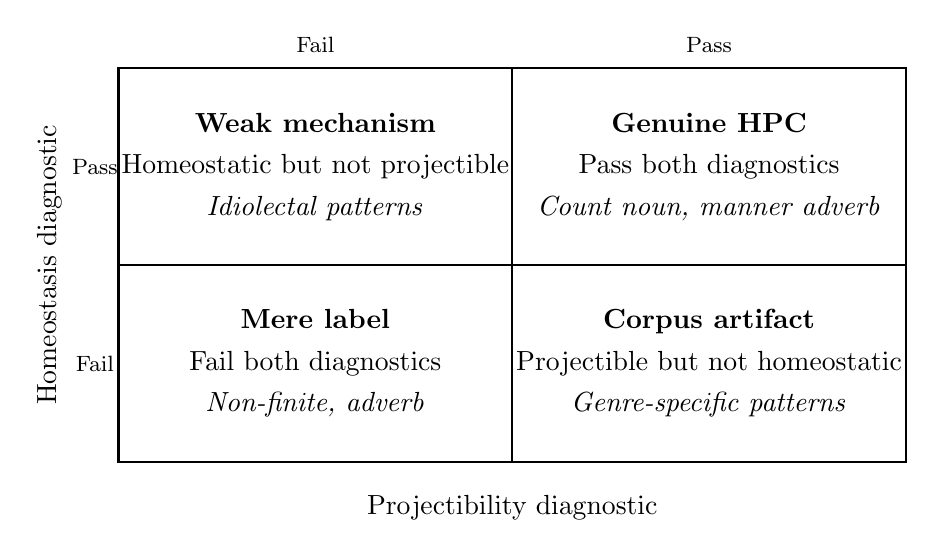
\begin{tikzpicture}[
    box/.style={rectangle, draw, minimum width=5cm, minimum height=2.5cm, align=center, font=\small},
    label/.style={font=\footnotesize\itshape}
]
% Grid
\draw[thick] (0,0) -- (10,0) -- (10,5) -- (0,5) -- cycle;
\draw[thick] (5,0) -- (5,5);
\draw[thick] (0,2.5) -- (10,2.5);

% Quadrant labels
\node[align=center] at (2.5,3.75) {\textbf{Weak mechanism}\\[3pt]Homeostatic but not projectible\\[3pt]\textit{Idiolectal patterns}};
\node[align=center] at (7.5,3.75) {\textbf{Genuine HPC}\\[3pt]Pass both diagnostics\\[3pt]\textit{Count noun, manner adverb}};
\node[align=center] at (2.5,1.25) {\textbf{Mere label}\\[3pt]Fail both diagnostics\\[3pt]\textit{Non-finite, \enquote{adverb}}};
\node[align=center] at (7.5,1.25) {\textbf{Corpus artifact}\\[3pt]Projectible but not homeostatic\\[3pt]\textit{Genre-specific patterns}};

% Axis labels
\node[rotate=90, anchor=south] at (-0.6,2.5) {Homeostasis diagnostic};
\node[anchor=north] at (5,-0.3) {Projectibility diagnostic};
\node at (2.5,5.3) {\footnotesize Fail};
\node at (7.5,5.3) {\footnotesize Pass};
\node at (-0.3,3.75) {\footnotesize Pass};
\node at (-0.3,1.25) {\footnotesize Fail};
\end{tikzpicture}
\caption{The two-diagnostic matrix. Only categories in the upper-right quadrant are genuine HPC kinds. The three failure modes occupy the other quadrants: thin categories (upper-left: mechanism without prediction), fat/negative categories (lower-left: neither mechanism nor prediction), and corpus artifacts (lower-right: prediction without mechanism).}
\label{fig:diagnostic-matrix}
\end{figure}

\subsection{The grain question}

One more trap before the case studies: the problem of grain. Even when we have genuine HPCs, we often group them into larger systems labelled \enquote{Grammar} or \enquote{Language.} Is \term{English Morphosyntax} an HPC kind?

The temptation is to say yes. It's stable, it's learned, it's maintained. But this is the \term{Madagascar fallacy}. Biological species are the paradigmatic HPC kinds. \textit{Lemur catta} (the ring-tailed lemur) is a homeostatic cluster maintained by interbreeding, shared ecology, and genetic transmission. But consider \enquote{the fauna of Madagascar.} It is a stable collection of animals. It is distinct from the fauna of Australia. It has a causal history (isolation). But \enquote{the fauna of Madagascar} is not itself a species. It is an \emph{ecosystem} of species. There is no single mechanism that maintains \enquote{the fauna} as a unit; there are thousands of mechanisms maintaining the individual populations that comprise it.

Language is an ecosystem. The HPCs are the individual form-meaning pairings~-- the constructions, the lexemes, the phonemes~-- not the grammar as a whole. The failure modes below apply at that level: we ask whether \term{adverb} is a kind, not whether \term{English} is. Section~\ref{sec:8:grain} returns to this question; for now, the point is that grain matters. A category can be too thin, too fat, too negative~-- or simply at the wrong level of analysis.


\section{Thin clustering: The smoke ring}
\label{sec:8:thin}

The first pattern is the category that barely exists.

A \term{thin} category is one where the signal exists~-- speakers recognise it, linguists name it~-- but the property cluster is ghostly. There is no robust homeostatic loop maintaining it. It is a \enquote{smoke ring}: it has structure, but that structure is ephemeral, typically generated by a transient convergence of other mechanisms rather than a dedicated feedback loop of its own.

Thin categories miss the homeostasis diagnostic. We cannot name their stabilisers~-- because there are none, or none sufficient to produce stable clustering.

\subsection{The nonce word test}

\citet{miller2021} provides a useful operationalisation. Whether a novel form counts as a \enquote{word-kind} depends on whether stable mechanisms~-- internal (cognitive) and external (social)~-- have emerged to maintain it. Consider \term{cromulent}, coined for a 1996 television episode to mean \enquote{acceptable, fine.}

Does \term{cromulent} exist as a word? Miller's answer: ask about the mechanisms. Are there internal cognitive structures ensuring that speakers produce the form consistently? Are there social norms ensuring that speakers use it in stable, predictable ways? For Simpsons fans, yes~-- in certain communities, the form is well-established, with consistent pronunciation and stable meaning. For the general population, no~-- the form remains an in-joke, not a general-purpose word.

The point is not that \term{cromulent} is \enquote{real} or \enquote{fake} but that its status depends on which mechanisms have stabilised where. A form can be an HPC kind in one speech community and a thin pattern in another. The question is always: what maintains it?

The nonce word test generalises: a category is thin when the mechanisms haven't stabilised. This can happen for new forms (nonce coinages), rare forms (idiolectal oddities), or forms maintained only by accident (spillover from other patterns).

\subsection{Case study: \textit{Whose}-stranding}

English allows preposition stranding in \textit{wh}-questions: \mention{Who did you talk to?} instead of \mention{To whom did you talk?} This is robustly maintained. But stranding extends, at very low frequency, to the possessive determiner \textit{whose}:

\begin{quote}
\mention{the guy whose I borrowed car}\\
\mention{the man whose they took wallet}
\end{quote}

This pattern exists. It is attested in corpus data and sociolinguistic interviews. It is reproducible: speakers who produce it don't treat it as an error. But it is thin.

The frequency is vanishing: roughly 1 per 100 million words~-- so rare that no child could acquire it from exposure alone. There is no social indexing: \textit{whose}-stranding signals nothing about the speaker's identity, register, or stance. There is no functional niche: pied-piping (\mention{whose car I borrowed}) or paraphrase (\mention{the guy I borrowed the car from}) serve the same function without the processing complexity.

Apply the homeostasis diagnostic: can we name the stabilisers?

\begin{itemize}
    \item \textbf{Acquisition:} Fails. Insufficient tokens for learners to extract a rule.
    \item \textbf{Entrenchment:} Fails. No speaker uses it frequently enough for lexeme-level strengthening.
    \item \textbf{Social indexing:} Fails. Carries no sociolinguistic meaning.
    \item \textbf{Functional pressure:} Fails. Competitors serve the function equally well.
\end{itemize}

What generates \textit{whose}-stranding is not a dedicated mechanism but a \term{spillover effect}. The general stranding parameter in English applies to \textit{wh}-phrases; \textit{whose} is a \textit{wh}-phrase; therefore speakers occasionally strand it. The pattern is a side-effect of more robust mechanisms, not a target of maintenance in its own right.

Compare to robust stranding: \mention{Who did you see?} This form is maintained by every mechanism on the list. Acquisition data shows children produce it early. Frequency is high. Social norms reinforce it (formal registers prefer pied-piping, informal registers prefer stranding~-- there's indexicality). Functional load is substantial. Object \textit{wh}-stranding is an HPC; \textit{whose}-stranding is its smoke ring~-- cast off by the same dynamics but lacking the immune system to persist independently.

The perturbation test makes this vivid. If English lost \textit{whose}-stranding tomorrow~-- if speakers simply stopped producing it~-- no feedback loop would kick in to restore it. No acquisition pressure, no social correction, no functional gap. It would vanish without a trace. A genuine HPC resists perturbation; a smoke ring dissipates.

Robust HPCs are \emph{attractors}: the mechanisms pull deviant instances back toward the cluster. Thin kinds are \emph{saddle points}: stable only while nothing disturbs them, collapsing under any perturbation. This is what it means to fail the homeostasis diagnostic. The pattern is real~-- it can be observed, described, named~-- but the causal structure that would maintain it is absent. We have a label without a kind.

\section{Fat clustering: The wastebasket}
\label{sec:8:fat}

The second pattern is the opposite of thinness: not too little mechanism, but too many pulling in different directions.

A \term{fat} category is a label that lumps distinct causal clusters into a single bin. The analyst treats them as one~-- usually for \enquote{wastebasket} reasons, where the category is defined residually: \enquote{everything that isn't X goes here.} But the mechanisms maintaining the subgroups are radically different. Fat categories miss the projectibility diagnostic: learning one subclass doesn't let you predict others.

Fat categories create an illusion of understanding. We have a label, so we act as if we have a kind. But the label masks the heterogeneity. Seeing \term{adverb} on the page, we assume there's something that makes all adverbs adverbs~-- some shared mechanism or property cluster. When we look for it, we find only the absence of other features.

Fat categories arise when different causal clusters get lumped under the same label for non-causal reasons. The analyst's goal~-- taxonomic completeness~-- treats manner adverbs and degree words alike because both are \enquote{modifiers that aren't adjectives.} But in causal terms, they occupy different regions with different mechanisms.

\subsection{Case study: The \term{Adverb}}

Try this: \mention{She ran quickly.} Now try: *\mention{She ran very.} Both \mention{quickly} and \mention{very} are adverbs~-- the same part of speech, according to every grammar textbook. Yet one sentence is grammatical and the other isn't. What went wrong?

The answer reveals everything about fat categories. \term{Adverb} doesn't name a natural kind; it names a filing cabinet where grammarians store everything that modifies but isn't an adjective. The items in the drawer have almost nothing in common~-- and when we try to generalise across them, the predictions collapse.

The traditional category \term{adverb} is the paradigmatic fat category~-- what introductory textbooks call the \enquote{dustbin of the parts of speech.} Look inside and you'll find at least three distinct clusters, each with its own mechanisms.

\textbf{Manner adverbs} (\mention{quickly}, \mention{carefully}, \mention{silently}) form an open class, productively derived from adjectives via \textit{-ly} suffixation. They integrate into the VP, favouring VP-final position: \mention{She ran quickly.} What maintains them? Productive derivational morphology (the \textit{-ly} rule applies to novel adjectives), VP-internal syntactic licensing, and early acquisition of the adjective-to-adverb mapping.

\textbf{Degree words} (\mention{very}, \mention{quite}, \mention{rather}) form a closed class~-- a handful of items, fixed in the lexicon. They modify adjectives and other adverbs, never verbs directly: \mention{very tall}, \mention{quite slowly}, but not *\mention{She ran very.} What maintains them? High-frequency entrenchment (each is memorised, not derived), functional specificity (a narrow scalar-modification niche), and closed-class conservatism (no productive rule generates new degree words).

\textbf{Sentence adverbs} (\mention{unfortunately}, \mention{frankly}, \mention{obviously}) scope over propositions, expressing speaker attitude. Prosodically, they're detached~-- set off by commas, placed sentence-initially. Syntactically, they're peripheral to the VP. What maintains them? Discourse-level alignment (speaker-stance marking), prosodic separation, and pragmatic function distinct from event modification.

Three clusters, three sets of mechanisms. The label \term{adverb} lumps them only because they share a negative property: they're modifiers that aren't adjectives. That's why \mention{quickly} and \mention{very} can't swap positions~-- they live in different rooms of the filing cabinet, maintained by different causal processes.

\subsection{The projectibility failure}

Now apply the projectibility diagnostic. Train on manner adverbs; test on degree words.

\citet[45]{ernst2002syntax} demonstrates that predicational adverbs show a rigid ordering hierarchy~-- discourse-oriented > evaluative > modal > evidential > subject-oriented > manner~-- and that only manner adverbs may appear to the right of the verb. These aren't stylistic preferences; they're grammatical constraints. Learning the distribution of one class tells you nothing about another.

Learning the distribution of \mention{quickly}~-- that it can appear sentence-finally (\mention{She ran quickly})~-- generates a prediction for other \enquote{adverbs.} But the prediction fails catastrophically for degree words: *\mention{It was good very.} And for modal adverbs: *\mention{She left probably.} The pattern doesn't travel.

Conversely, learning that \mention{very} requires an adjective host~-- \mention{very tall}~-- generates a prediction that fails for sentence adverbs: \mention{Unfortunately, she left} has no adjective host at all.

The projectibility test delivers a clear negative. The category \term{adverb} doesn't support cross-subclass generalisation. What you learn about one subtype tells you nothing reliable about another. This is diagnostic of a fat category: the label groups items that were never maintained by shared mechanisms.

Fat categories arise because exhaustive taxonomy requires a home for everything. If you need every word to belong to exactly one part of speech, and you've already defined noun, verb, adjective, preposition, determiner, and conjunction, then \enquote{everything left over} must go somewhere. \term{Adverb} is that somewhere. The label groups items that are \enquote{close} only in the analyst's filing system. In terms of the mechanisms that maintain them, manner adverbs and degree words are far apart. The label is a convenience, not a kind.

The maintenance view gives clear guidance when you diagnose a fat category: decompose. \term{Adverb} is not an HPC. But \term{Manner Adverb}, \term{Degree Word}, and \term{Sentence Adverb} may be. They're the genuine clusters lurking inside the wastebasket. The lump is a taxonomic fiction; the components are causally real. This doesn't mean abolishing the term~-- \term{adverb} remains useful for some purposes~-- but it means recognising that the term names an epistemic kind, not a natural kind. When you're doing HPC analysis, look below the lump.

A note of sympathy for the original grammarians. They weren't being lazy. Imagine standing in front of the scattered words that aren't nouns or verbs, facing the pedagogical demand to say what they are. Students need labels. Textbooks need categories. The pressure to provide \emph{some} answer~-- any answer~-- is real. Reaching for \term{adverb} was not a failure of intelligence but a response to genuine classificatory pressure. The maintenance view doesn't condemn that move; it just asks what we can learn from it. The answer is that exhaustive taxonomy and natural-kind discovery are not the same enterprise, and sometimes they pull in different directions.

\section{Negative categories: The complement class}
\label{sec:8:negative}

The third pattern is the most categorical: the category defined by what it is not.

A \term{negative} category is a complement class: \enquote{everything that isn't X.} In set theory, complements are well-behaved~-- the complement of a set is precisely defined. In causal mechanism terms, they're incoherent. There is no such thing as a \enquote{homeostatic property cluster of absence.} The absence of a property is typically not a property, and certainly not one that mechanisms can stabilise.

Negative categories miss both diagnostics. They miss projectibility because members share no positive properties to generalise from. They miss homeostasis because no mechanism can maintain \enquote{lacking X}~-- what would such a mechanism even look like?

\subsection{Case study: The \term{Non-finite}}

Consider the category \term{non-finite verb}. In traditional grammar~-- and in most contemporary frameworks~-- it groups:

\begin{itemize}
    \item \textbf{Infinitives:} \mention{to eat}, \mention{to run}
    \item \textbf{Bare stems:} \mention{eat}, \mention{run} (after modals: \mention{can eat})
    \item \textbf{Past participles:} \mention{eaten}, \mention{run}
    \item \textbf{Gerund-participles:} \mention{eating}, \mention{running}
\end{itemize}

What do they share? The standard answer is negative: they lack tense marking, they lack agreement (mostly), they cannot head a main clause (mostly). They're grouped by absence.

But look at their positive properties~-- their syntactic environments, their maintaining mechanisms~-- and they're radically different animals.

\textbf{Infinitives} appear in control contexts (\mention{I want to leave}), as purposive adjuncts (\mention{I came to help}), as subjects (\mention{To err is human}). What maintains them? Control verb selection (verbs like \textit{want}, \textit{try}, \textit{hope} select infinitival complements), purposive adverbial licensing, and historical entrenchment of the \textit{to}-infinitive construction.

\textbf{Bare stems} appear after modal auxiliaries (\mention{can eat}, \mention{will run}), in subjunctive mandatives (\mention{I insist that she leave}), and after perception and causative verbs (\mention{I saw her leave}). Different mechanisms: the modal auxiliary system, the mandative construction with its own acquisition path, and ECM licensing for perception verbs.

\textbf{Past participles} appear in the perfect (\mention{has eaten}), the passive (\mention{was eaten}), and as adjectival modifiers (\mention{the broken window}). Different mechanisms again: the perfect auxiliary system, the passive voice construction, and adjectival conversion.

\textbf{Gerund-participles} appear in the progressive (\mention{is eating}), as nominalisations (\mention{Eating is fun}), and as participial adjuncts (\mention{Walking home, I saw a fox}). Still different mechanisms: progressive aspect construction, nominalisation patterns, and participial adjunct licensing.

Four forms, four sets of environments, four sets of mechanisms. The only thing they share is a negative: lacking tense.

\subsection{Both diagnostics fail}

Now apply the tests.

\textbf{Projectibility:} If you learn the distribution of infinitives~-- where \mention{to eat} can appear~-- does that help you predict the distribution of past participles? No. Knowing that \mention{to leave} follows \textit{want} tells you nothing about where \mention{left} (the past participle) can appear. The syntactic environments don't overlap; the predictions don't transfer. The category doesn't project.

\textbf{Homeostasis:} Can we name a mechanism that maintains infinitives and gerund-participles as similar to each other? No. The perfect auxiliary system has nothing to do with the progressive auxiliary system~-- except that both happen to select forms lacking tense. There's no feedback loop that keeps non-finites together as a kind. They're grouped only by failing to be finite.

Negative categories show this most starkly. The analyst's need for exhaustive taxonomy requires every verb form to belong to a category, and \enquote{everything that's not finite} must go somewhere. But the property structure is empty. There's no positive cluster, only the absence of tense and agreement. This is classification by exclusion, not by mechanism. The label \term{non-finite} organises the analyst's files; it doesn't track causal structure.

When you diagnose a negative category, the guidance is clear: don't treat it as a kind. This doesn't mean the term is useless~-- \term{non-finite} correctly identifies forms that contrast with finites~-- but it means recognising that the term is a taxonomic convenience, not a natural kind. The genuine HPCs are the sub-constructions: \term{infinitival complement}, \term{perfect construction}, \term{progressive construction}, \term{participial adjunct}. Each has its own cluster, its own mechanisms, its own projectibility. The umbrella term names a residual class, not a causal unity.

\section{The grain of analysis}
\label{sec:8:grain}

The grain question previewed in §\ref{sec:8:diagnostics} deserves more detail. We said language is an ecosystem~-- but which are the species?

\subsection{Constructions are the kinds}

The HPCs are the \emph{components}, not the whole.

The phoneme /θ/ is an HPC (stabilised by articulatory targets and contrasts). The word \term{\textit{dog}} is an HPC (stabilised by lexical entrenchment). The construction \term{\textit{let alone}} is an HPC (stabilised by a cue bundle of string, syntax, and scalar semantics).

But \enquote{English Grammar} is just the island where they all live. It is the \term{constructicon}~-- the population of constructional species inhabiting a speech community. 

This gives us the answer to the grain question. The level of analysis where HPC theory applies is the level of the \term{individual form-meaning pairing}. 
\begin{itemize}
    \item \term{Noun} is likely a fat category (an umbrella for many specific nominal constructions).
    \item \term{Count Noun} is a plausible HPC (a specific sub-family of constructions with shared maintenance).
    \item \term{The construction \textit{let alone}} is definitely an HPC.
    \item \term{English} is not an HPC; it's the fauna.
\end{itemize}

The discipline of the framework forces us to go local. We find the mechanisms where they live: in the specific transmission of specific patterns. When we lump too high, we lose the causal thread.

\section{Methodological implications}
\label{sec:8:implications}

If we adopt this discipline, the landscape of linguistics looks different. The framework doesn't just identify failures~-- it tells us what to do about them.

\subsection{What to do when you diagnose failure}

Each failure mode has a corresponding response.

\textbf{When you diagnose thinness:} Stop treating the pattern as a category. \textit{Whose}-stranding isn't a construction to be explained; it's a spillover effect to be noted and set aside. Thin patterns don't need theoretical treatment because they lack the causal structure that would make treatment meaningful. Document them, but don't reify them.

\textbf{When you diagnose fatness:} Decompose. \term{Adverb} isn't a kind; \term{Manner Adverb}, \term{Degree Word}, and \term{Sentence Adverb} might be. The genuine HPCs are lurking inside the wastebasket. Your job is to find them~-- to identify the sub-clusters that actually pass the diagnostics. The lumped label may remain useful for pedagogy or exposition, but it shouldn't guide theoretical inference.

\textbf{When you diagnose negativity:} Reframe. \term{Non-finite} names a contrast, not a unity. Replace it with positive categories~-- \term{infinitival complement}, \term{perfect construction}, \term{progressive construction}~-- that actually have mechanisms to maintain them. The negative label organises your files; it doesn't track causal structure.

\subsection{For typology}

The framework reframes cross-linguistic comparison.

We stop asking whether \term{Subject} is a universal category~-- a question that invites endless definitional dispute. Instead, we ask: is the category \term{Subject} in Language L maintained by the same mechanisms as in Language M?

Usually, the answer is no. English subjects are maintained by agreement morphology, fixed word order, and nominative case marking. Tagalog \enquote{subjects} (if that's even the right term) are maintained by voice morphology and discourse-role assignment~-- entirely different mechanisms. They may look alike~-- both occupy some privileged argument position~-- but they're distinct HPCs, convergent solutions to different functional pressures.

This is convergent evolution, not shared identity. The sameness of the label doesn't guarantee sameness of the kind. To test cross-linguistic identity, you need to show shared mechanisms, not just shared features.

\subsection{For theory}

The framework shifts the burden of proof.

Labels without mechanisms are descriptive, not explanatory. If you claim that \term{voice} is a category in Language L, you need more than distributional evidence. You need to identify the mechanisms maintaining it~-- the acquisition pathways, the frequency effects, the functional pressures that keep the pattern stable.

This isn't a higher bar; it's a different bar. The framework doesn't demand more evidence; it demands a different kind of evidence. Mechanism identification becomes the theoretical goal, not just category identification.

\subsection{For methodology}

Falsifiability is built in.

The two-diagnostic test gives a decision procedure: apply projectibility and homeostasis criteria; if the pattern fails, it's not an HPC kind. This creates a research programme with clear success conditions. You can be wrong in a way that's detectable~-- and that's what makes the framework scientific.

The framework also explains gradience. Degrees of projectibility~-- strong at the core, weak at the periphery~-- aren't noise to be averaged away. They're signal: the signature of mechanisms operating at different strengths across the category. Peripheral variability tells you something about the causal structure.

\subsection{Looking forward}

This chapter has provided the discipline. It has shown what failure looks like~-- thin, fat, negative~-- and how to diagnose it using the two-diagnostic test. The framework can now be applied.

The same diagnostics~-- projectibility and the presence of stabilising mechanisms~-- apply at the cross-linguistic level. Comparative concepts like \textsc{noun} and \textsc{adjective} can be diagnosed as thin (diagnostics fail across families), fat (the category lumps distinct phenomena), or negative (defined by what it's not). Chapter~\ref{ch:what-changes} develops this typological implication; \textcite{reynolds2025comparanda} provides the formal framework.

Part III applies it. Countability offers an HPC that passes both diagnostics. Definiteness presents a case where form and meaning may constitute separate, overlapping HPCs. Word classes return us to traditional categories~-- asking which survive the test and which decompose under pressure. And the final chapter asks whether the framework scales~-- from phonemes to constructions to \enquote{the grammar} itself.

The question is no longer \enquote{Is this a category?} but \enquote{Is this a kind?} The diagnostics give us a way to answer.

